\documentclass[12pt]{article}
\usepackage[margin=2.5cm]{geometry}
\usepackage{tikz}
\usepackage{amsmath}
\setlength{\parindent}{0pt}
\setlength{\parskip}{0.75em}



\title{Chapter 2: Kinematics}
\author{İskender Yalçınkaya, PhD}
\date{\today}

\begin{document}
\maketitle
\section{Notion of a Particle}
A \emph{particle} is a body whose size and shape are not important for the problem at hand. In other words, a particle is a body that can be treated as a point mass. The motion of a particle is described by its position, velocity, and acceleration as functions of time. For example, planets can be treated as particles when studying their motion around the sun, even though they have size and shape. But when studying the tidal waves on earth and the tornadoes in the atmosphere, the size and shape of the earth is important, and they cannot be treated as particles.

Mathematically, a particle is a point in the space with an associated mass. Therefore, if one has to define a density function for a point particle which is located at $\mathbf{r}_0$, it would look like:
\[
\rho(\mathbf{r}) =
\begin{cases}
\infty, & \mathbf{r} = \mathbf{r}_0,\\[4pt]
0, & \mathbf{r} \neq \mathbf{r}_0.
\end{cases}
\]


\section{The Position Vector}
The position of a particle is described by a vector called the \emph{position vector}:
\begin{equation}
\mathbf{r}(t) = x(t) \mathbf{i} + y(t) \mathbf{j} + z(t) \mathbf{k}
\end{equation}
where $x(t)$, $y(t)$, and $z(t)$ are the coordinates of the particle in a Cartesian coordinate system, and $\mathbf{i}$, $\mathbf{j}$, and $\mathbf{k}$ are the unit vectors in the $x$, $y$, and $z$ directions, respectively. The position vector points from the origin of the coordinate system to the position of the particle at time $t$. The magnitude of the position vector represents the distance of the particle from the origin, and its direction represents the direction of the particle from the origin. The position vector is a function of time, and it can be used to describe the motion of the particle in space. The position vector can also be expressed in terms of spherical or cylindrical coordinates, depending on the problem at hand. 


\begin{figure}[ht]
\centering
\begin{tikzpicture}[>=stealth, scale=1.2]

    % Axes
    \draw[->] (-0.3,0) -- (5,0) node[right] {$x$};
    \draw[->] (0,-0.3) -- (0,4) node[above] {$y$};

    % Particle
    \fill (3.5,2.5) circle (2pt) node[above right] {Particle};

    % Position vector
    \draw[->, thick] (0,0) -- (3.5,2.5)
        node[midway, above left] {$\mathbf{r}(t)$};

    % Coordinates
    \draw[dashed] (3.5,0) -- (3.5,2.5);
    \draw[dashed] (0,2.5) -- (3.5,2.5);

    % Coordinate labels
    \node[below] at (3.5,0) {$x(t)$};
    \node[left] at (0,2.5) {$y(t)$};

    % Origin
    \node[below left] at (0,0) {$O$};

\end{tikzpicture}
\caption{The position vector $\mathbf{r}(t)$ of a particle in a two-dimensional Cartesian coordinate system.}
\label{fig:position_vector}
\end{figure}


\section{The Displacement Vector}
What happens if a particle moves from one position $r_1(t_1)$ to another position $r_2(t_2)$? The displacement of a particle is described by a vector called the \emph{displacement vector}. It is defined as the change in position of the particle, and is given by the difference between the final position vector and the initial position vector:
\begin{equation}
\Delta \mathbf{r} = \mathbf{r}_2 (t_2) - \mathbf{r}_1 (t_1)
\end{equation}

The displacement vector points from the initial position to the final position, and its magnitude represents the distance traveled by the particle in a straight line. The displacement vector is independent of the path taken by the particle, and only depends on the initial and final positions.

\begin{figure}[h]
\centering
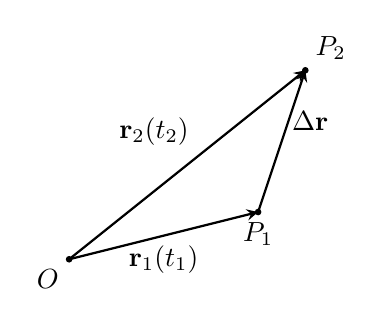
\begin{tikzpicture}[>=stealth, thick, scale=0.6]

    % Points
    \coordinate (O)  at (0,0);
    \coordinate (P1) at (4,1);
    \coordinate (P2) at (5,4);

    % Position vector r_1
    \draw[->] (O) -- (P1)
        node[midway, below] {$\mathbf{r}_1(t_1)$};

    % Position vector r_2
    \draw[->] (O) -- (P2)
        node[pos=0.55, above left] {$\mathbf{r}_2(t_2)$};

    % Displacement vector
    \draw[->] (P1) -- (P2)
        node[midway, above right] {$\Delta\mathbf{r}$};

    % Points
    \fill (O) circle (2pt) node[below left] {$O$};
    \fill (P1) circle (2pt) node[below] {$P_1$};
    \fill (P2) circle (2pt) node[above right] {$P_2$};

\end{tikzpicture}
\caption{Position vectors and displacement vector.}
\label{fig:position_displacement}
\end{figure}

If we simple subtract $\mathbf{r}_1$ from $\mathbf{r}_2$ by using the head to tail method, the resulting vector would be in some direction starting from the origin. But the displacement vector is defined as the vector that starts from the initial position and ends at the final position. Therefore, we need to translate the vector $\mathbf{r}_1$ to the point $\mathbf{r}_2$ in order to find the displacement vector $\Delta \mathbf{r}$. This is shown in Figure \ref{fig:position_displacement}.


\section{The Velocity Vector}

The \emph{velocity} is defined as the change in position with respect to time. If the displacement of the particle is described by $\Delta \mathbf{r}$, can we define the velocity as follows?

\[
\mathbf{v}\overset{?}{=}\frac{\Delta \mathbf{r}}{\Delta t}
\]
What does this actually mean? Maybe the particle moved between the time interval $t_2-t_1$ as shown in the following figure:

\begin{figure}[h]
\centering
This is a figure.
\end{figure}


Maybe the particle sped up during its motion or slowed down or maybe it took a brake for some time. We do not know. The information given to us in the beginning was only $\mathbf{r}_1(t)$ and $\mathbf{r}_2(t)$. Therefore, all we can say is how fast and in which direction the particle moved during $\Delta t$ ``on average''. Therefore, we define the \emph{average velocity vector} as
\[
\mathbf{v}_\text{avg}=\frac{\Delta \mathbf{r}}{\Delta t}
\]
It has the same direction as the displacement vector. If we are given the initial and final position vectors in component form as
\[
\mathbf{r}_1=x_1(t)\mathbf{i} + y_1(t)\mathbf{j} + z_1(t)\mathbf{k}
\]
\[
\mathbf{r}_2=x_2(t)\mathbf{i} + y_2(t)\mathbf{j} + z_2(t)\mathbf{k}
\]
\[
\Delta \mathbf{r} = \mathbf{r}_2 - \mathbf{r}_1 = [x_2(t)-x_1(t)]\mathbf{i} + [y_2(t)-y_1(t)]\mathbf{j} + [z_2(t)-z_1(t)]\mathbf{k}
\]
then the average velocity vector becomes
\[
\mathbf{v}_\text{avg}= \frac{\Delta x}{\Delta t}\mathbf{i}+\frac{\Delta y}{\Delta t}\mathbf{j}+\frac{\Delta z}{\Delta t}\mathbf{k}
\]

If we are interested in the velocity of the particle at a given time instead of the average velocity we should consider the behavior of $\mathbf{v}_\text{avg}$ when $\Delta t \rightarrow 0$. Therefore,

\[
\lim_{\Delta t \rightarrow 0} \mathbf{v}_\text{avg} = \lim_{\Delta t \rightarrow 0} \frac{\Delta x}{\Delta t}\mathbf{i}+\lim_{\Delta t \rightarrow 0}\frac{\Delta y}{\Delta t}\mathbf{j}+\lim_{\Delta t \rightarrow 0}\frac{\Delta z}{\Delta t}\mathbf{k},
\]
where we have the definition of derivatice for each term. Hence the velocity of a particle at time $t$ is defined as

\begin{equation}
    \mathbf{v}(t) = \frac{d}{dt}[x(t)]\mathbf{i}+\frac{d}{dt}[y(t)]\mathbf{j}+\frac{d}{dt}[z(t)]\mathbf{k},
\end{equation}

or in Newton's notation

\begin{equation}
    \mathbf{v}(t) = \dot{x}(t)\mathbf{i}+\dot{y}(t)\mathbf{j}+\dot{z}(t)\mathbf{k} = v_x(t)\mathbf{i}+v_y(t)\mathbf{j}+v_z(t)\mathbf{k}.
\end{equation}

The \emph{speed} of the particle is defined as the magnitude of the velocity vector:

\begin{equation}
    v(t) = |\mathbf{v}(t)|.
\end{equation}


\section{The Acceleration Vector}
to be continued...

\section{The Trajectory of a Particle}

The \emph{trajectory} of a particle is the path followed by the particle in space as time goes on.  




\end{document}
